\section{VL vom 23.~November 2010}

\subsection{Beispiele zur Semantik von FO}

\begin{itemize}
  \item Beispiel 1:\par
  $\Afrak$ 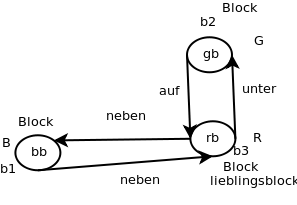
\includegraphics[width=6cm]{23_11_10_1.png}
  
  Zuweisung $\beta$: $\beta(x) = bb \qquad \beta(y) = gb \qquad \beta(z) = gb$
  % Absicht, da Beispielbelegung: \beta(y) = \beta(z)
  rb, gb, bb können nie in Formel auftauchen. Sind nur Semantik. Brauchen immer Konstantensymbol.

  \begin{align}
    \Afrak, \beta &\models \exists x.(R(x) \AND \forall y.(\text{auf}(y,x) \IMPL G(y))) && \text{Satz} \\
    \Afrak, \beta &\models \exists z.(\text{neben}(b_1,z) \AND \text{unter}(z,b_2))     && \text{Satz} \\
    \Afrak, \beta &\models \exists z.(\text{neben}(x,z) \AND \text{unter}(z,y))         && \text{kein Satz} \\
    \Afrak, \beta &\models x \not= b_2                                                  && \text{kein Satz} \\
    \Afrak, \beta &\models \forall x.(G(x) \OR B(x) \OR x = \text{lieblingsblock})      && \text{Satz}
  \end{align}
  
(24) - freie Variable x. Jetzt ist Zuweisung auch anzugucken. Vorher hat Blick auf die Struktur gereicht.

  \item Beispiel 2:\par
  $\mathfrak{N} = (\mathbb{N}, +, \cdot, 0, 1)$
  
  Sei $\beta$ beliebig. Dann gelten folgende Sätze:
  \begin{align}
    \mathfrak{N}, \beta &\models \forall x \forall x.(x+y=y+x) \\
                        & \qquad\text{(zur Vereinfachung: $a+b = +(a,b)$)} \notag\\
    \mathfrak{N}, \beta &\models \forall x.(\text{Prim}(x) \IMPL \exists y.(y>x \AND \text{Prim}(y))) \\
                        & \qquad\text{wobei $\text{Prim}(x) = \forall y,z.(x=y\cdot z \IMPL (y=1 \OR z=1))$} \notag\\
                        & \qquad\text{und $y>x = \exists z.(z\not=0 \AND x+z = y)$} \notag\\
    \mathfrak{N}, \beta &\stackrel{?}{\models} \forall x.(\text{Prim}(y) \AND \text{Prim}(y+z)) \\
                        & \qquad\text{wobei $y+z = (y+1)+1$} \notag\\
                        & \qquad\text{\enquote{Gibt es unendlich viele Primzahlzwillinge?}}\notag\\
                        & \qquad\text{(offenes Problem der Zahlentheorie)}\notag
  \end{align}
\end{itemize}

Satz: Formel ohne freie Variablen.\\
FO-Formel ist Eigenschaft von Struktur.\\
Koinzidenzlemma\\
\seeslide{32}

\subsection{Isomorphielemma}

\subsubsection{Beispiel}

$c_1, c_2  \in F^0(\tau) \qquad f \in F^1(\tau) \qquad R \in R^2(\tau)$

\begin{verbatim}
  Graph von Bernd tikzen
\end{verbatim}

\subsubsection{Beweis}

Wegen des Koinzidenzlemmas genügt es, zu zeigen:

Wenn $\mathcal{I}_\Afrak = (\Afrak,\beta)$ und $\mathcal{I}_\mathfrak{B} = (\mathfrak{B}, \beta)$ Interpretationen,
so dass $\beta'(x) = \pi(\beta(x))$ für alle $x\in VAR$, dann

\begin{itemize}
  \item[$(*)$] $\mathcal{I}_\Afrak \models \varphi$ für alle $\varphi \in FO(\tau)$
\end{itemize}

Man zeigt leicht per Induktion über die Struktur über die Struktur von t:

\begin{itemize}
  \item[$(**)$] $\beta'(t) = \pi(\beta(t))$ für alle $t \in T(\tau)$
\end{itemize}

Beweis von $(*)$ per Induktion über die Struktur von $\varphi$

\begin{itemize}
  \item \textbf{Induktionsanfang}
  \begin{enumerate}
    \item $\mathcal{I}_\Afrak \models t_1=t_2$\\
      gdw. $\beta(t_1) = \beta(t_2)$ (Semantik \enquote{=})\\
      gdw. $\pi(\beta(t_1)) = \pi(\beta(t_2))$ ($\pi$ injektiv)\\
      gdw. $\beta'(t_1) = \beta'(t_2)$ ($(**)$)\\
      gdw. $\mathcal{I}_\mathfrak{B} \models t_1=t_2$
    
    \item $\mathcal{I}_\Afrak \models P(t_1,\dots,t_k)$ \\
      gdw. $(\beta(t_1),\dots,\beta(t_k)) \in P^\Afrak$ \\
      gdw. $(\pi(\beta(t_1)),\dots,\pi(\beta(t_k))) \in P^\mathfrak{B}$ ($\pi$ isom.) \\
      gdw. $(\beta'(t_1),\dots,\beta'(t_k)) \in P^\mathfrak{B}$ \\
      gdw. $\mathcal{I}_\mathfrak{B} \models P(t_1,\dots,t_2)$
  \end{enumerate}
  
  \item \textbf{Induktionsschritt}
  \begin{enumerate}
    \item Fälle $\varphi = \NOT \psi$, $\varphi = \psi_1 \AND \psi_2$, $\varphi = \psi_1 \OR \psi_2$
      (Übung)
      
    \item $\mathcal{I}_\Afrak \models \exists x.\psi$ \\
      gdw. $(\Afrak, \beta[x/a]) \models \psi$ für ein $a \in A$\\
      gdw. $(B, \beta'[x/\pi(a)]) \models \psi$ für ein $a \in A$ (IV)\\
      gdw. $(B, \beta'[x/b]) \models \psi$ für ein $b \in B$ ($\pi$ surj.)\\
      gdw. $\mathcal{I}_B \models \exists x.\psi$
      
    \item Fall $\varphi = \forall x.\psi$ analog.
  \end{enumerate}
\end{itemize}
\qed


